\documentclass[addpoints,answers,12pt]{exam}

\usepackage{ifthen}

\ifthenelse{\equal{\includedsol}{solution}} 
{ 
\printanswers
} 
{ 
\noprintanswers
} 

% \documentclass[addpoints,answers,12pt]{exam}
\usepackage{graphicx}
% \usepackage{graphics}

% \usepackage{amsgen}
% \usepackage{amstext}
% \usepackage{amsmath}
% % \usepackage{amsthm}
% \usepackage{amsfonts}


\usepackage{latexsym}
\usepackage{amsgen}
\usepackage{amsmath}
\usepackage{amstext}
\usepackage{amscd}
\usepackage{amssymb}


\newcommand{\myinf}[3]{\inference[\textsc{#1}]{#2}{#3}}
\newcommand{\ndimpI}[2]{\myinf{$->$I}{#1}{#2}}
\newcommand{\ndcut}[2]{\myinf{Cut}{#1}{#2}}
\newcommand{\ndandE}[1]{\myinf{$\land$E}{}{#1}}
\newcommand{\ndimpE}[1]{\myinf{$->$E}{}{#1}}
\newcommand{\ndraa}[2]{\myinf{Raa}{#1}{#2}}
\newcommand{\ndbotE}[1]{\myinf{$\bot$E}{}{#1}}
\newcommand{\ndorE}[2]{\myinf{$\lor$E}{#1}{#2}}
\newcommand{\ndorI}[1]{\myinf{$\lor$I}{}{#1}}
\newcommand{\ndandI}[1]{\myinf{$\land$I}{}{#1}}
\setlength\answerclearance{0.6ex}

\firstpageheader{CSE
  344}{Final}{Name:\enspace\makebox[2in]{\hrulefill}}
\runningheader{CSE 344}{Final Examination}{March 14, 2012}


\newcommand{\eat}[1]{}

\begin{document}

\title{CSE 344 Final Examination} \author{} \date{March 14, 2012,
  8:30am - 10:20am}

\maketitle

\begin{center}
{
\vspace{1cm}

Name:\enspace\makebox[3in]{\hrulefill}

\vspace{1cm}

\gradetable
}
\end{center}

\begin{itemize}
\item This exam is a closed book exam.
\item You have 1h:50 minutes; budget time carefully.
\item Please read all questions carefully before answering them.
\item Some questions are easier, others harder; if a question sounds
  hard, skip it and return later.
\item Good luck!
\end{itemize}

\newpage


\begin{questions}

\section{SQL, Relational Calculus, Relational Algebra}


\question (\totalpoints\ \points) 

\label{q:sql}


\noindent The following database constains information about email messages in a
large organization:

\begin{tabular}{l}
\texttt{Person(\underline{pid},name)} \\
\texttt{Email(\underline{eid}, pidFrom, tid, body, length)} \\
\texttt{EmailTo(eid,pidTo)}
\end{tabular}

Where:
\begin{itemize}
\item  \texttt{Person.pid} and \texttt{Email.eid} are keys.
\item \texttt{Email.pidFrom} and \texttt{EmailTo.pidTo} are foreign keys to \texttt{Person}.
\item \texttt{EmaiTo.eid} is a foreign key to \texttt{Email}.
\item Every email may be sent to several recipients, stored in the
  \texttt{EmailTo} table.
\item \texttt{tid} represents the thread to which the email belongs.
\end{itemize}


\begin{parts}
  \part[10] Write the SQL statements that define the relational schema
  for this database.  Assume that \texttt{pid}'s and \texttt{eid} s
  are integers, and \texttt{name} and \texttt{body} are character
  strings (choose an appropriate length).

\underline{\bf Answer} (write  a SQL statement):


\vfill

\begin{solution}
\begin{verbatim}
create table Person(
  pid int primary key,
  name varchar(20));
create table Email(
  eid int primary key,
  pidFrom int references Person,
  tid int,
  body varchar(1024),
  length int);
create table EmailTo(
  eid int references Email,
  pidTo int references Person);
\end{verbatim}
Notes:
\begin{itemize}
\item 1 point off for each missing key or foreign key.
\end{itemize}
\end{solution}

\newpage

{\scriptsize
\hfill
\begin{tabular}{l}
\texttt{Person(\underline{pid},name)} \\
\texttt{Email(\underline{eid}, pidFrom, tid, body, length)} \\
\texttt{EmailTo(eid,pidTo)}
\end{tabular}
}


  \part[10] For each email thread, compute the total number of
  distinct recipients of emails in that thread.  For example, if the
  thread contains 100 emails, and all emails went to only one
  recipient, then your query should answer 1 for that thread id.

\vspace{1cm}

\underline{\bf Answer} (write  a SQL statement):

\vfill

\begin{solution}
\begin{verbatim}
select e.tid, count(distinct e2.pidTo)
from Email e, EmailTo e2
where e.eid = e2.eid
group by e.tid
\end{verbatim}
Notes:
\begin{itemize}
\item Left outer join is OK (even preferable).
\item 2 points off if \texttt{count(*)} instead  \texttt{count(distinct \ldots)}.
\item 1 point off for nested query with \texttt{select distinct} (if correct).
\item 1 point off if joined unnecessarily with \texttt{Person}.
\end{itemize}
\end{solution}

\newpage

{\scriptsize
\hfill
\begin{tabular}{l}
\texttt{Person(\underline{pid},name)} \\
\texttt{Email(\underline{eid}, pidFrom, tid, body, length)} \\
\texttt{EmailTo(eid,pidTo)}
\end{tabular}
}

\part[10] A {\em circle} is a set of three users $a$, $b$, $c$ such
that $a$ sent an email to $b$, $b$ sent an email to $c$, $c$ sent an
email to $a$, and all these three emails are in the same thread.
Write a SQL query that computes the total number of circles in the
database.

\vspace{1cm}

\underline{\bf Answer} (write a SQL query):


\vfill

\begin{solution}
\begin{verbatim}
select count(*)
from email e1, emailTo t1, email e2, emailTo t2, email e3, emailTo t3
where e1.eid = t1.eid and t1.pidTo = e2.pidFrom
  and e2.eid = t2.eid and t2.pidTo = e3.pidFrom
  and e3.eid = t3.eid and t3.pidTo = e1.pidFrom
  and e1.tid = e2.tid and e2.tid = e3.tid;
\end{verbatim}
Notes:
\begin{itemize}
\item 1 point off if joined unnecessarily with \texttt{Person}.
\item 2 points off for missing join on \texttt{tid}, and similarly for
  \texttt{eid}.
\item 5 points off or more for nested queries (most of which don't
  work).
\end{itemize}
\end{solution}


\newpage

{\scriptsize
\hfill
\begin{tabular}{l}
\texttt{Person(\underline{pid},name)} \\
\texttt{Email(\underline{eid}, pidFrom, tid, body, length)} \\
\texttt{EmailTo(eid,pidTo)}
\end{tabular}
}

\part[10] A {\em spammer} is a person who has sent at least one email
in every thread.  Write a SQL query to find all spammers.  Your query
should return the spammer's pid and their name.

\vspace{1cm}

\underline{\bf Answer} (write a SQL query):

\vfill

\begin{solution}
{\scriptsize
I first write it in the Relational Calculus, then remove universal quantifiers:
\begin{align*}
  Q(pid,n) & = \texttt{Person}(pid,n) \wedge (\forall eid_1,pidf_1,tid,b_1,l_1. \texttt{Email}(eid_1,pidf_1,tid,b_1,l_1) \Rightarrow \exists eid_2,b_2,l_2.\texttt{Email}(eid_2,pid,tid,b_2,l_2))\\
   & = \texttt{Person}(pid,n) \wedge \not (\exists eid_1,pidf_1,tid,b_1,l_1. \texttt{Email}(eid_1,pidf_1,tid,b_1,l_1) \wedge\not\exists eid_2,b_2,l_2.\texttt{Email}(eid_2,pid,tid,b_2,l_2))\\
\end{align*}
Next, datalog:
\begin{verbatim}
T(pid, tid) :- Email(eid2,pid,tid,b2,l2)
K(pid)      :- Person(pid,-), Email(eid1,pidf1,tid,b1,l1), not T(pid,tid)
Q(pid)      :- Person(pid,n), not K(pid)
\end{verbatim}
The predicate \texttt{Person(pid,-)} in the definition of \texttt{K}
is introduced in order to make the rule safe.  We now translate to
SQL, and may remove that predicate:

\begin{verbatim}
select p.pid
from Person p
where not exists (select *
                  from Email e1
                  where not exists (select *
                                    from Email e2
                                    where e2.pidFrom = p.pid and e2.tid=e1.tid));
\end{verbatim}
}

Notes:
\begin{itemize}
\item 6 points credit for one correct negation (\texttt{Person not in \ldots}).
\end{itemize}
\end{solution}

\newpage

{\scriptsize
\hfill
\begin{tabular}{l}
\texttt{Person(\underline{pid},name)} \\
\texttt{Email(\underline{eid}, pidFrom, tid, body, length)} \\
\texttt{EmailTo(eid,pidTo)}
\end{tabular}
}

\part[10]  Write a query plan in the extended relational algebra that
computes the following query:

\begin{verbatim}
select e1.pidFrom, count(*)
from Email e1, EmailTo t1, Email e2
where e1.eid = t1.eid and t1.pidTo = e2.pidFrom
group by e1.pidFrom
having max(e2.length) < 1000;
\end{verbatim}

\underline{\bf Answer} (write a  query plan; you may draw it as a tree):

\vfill

\begin{solution}

  \centerline{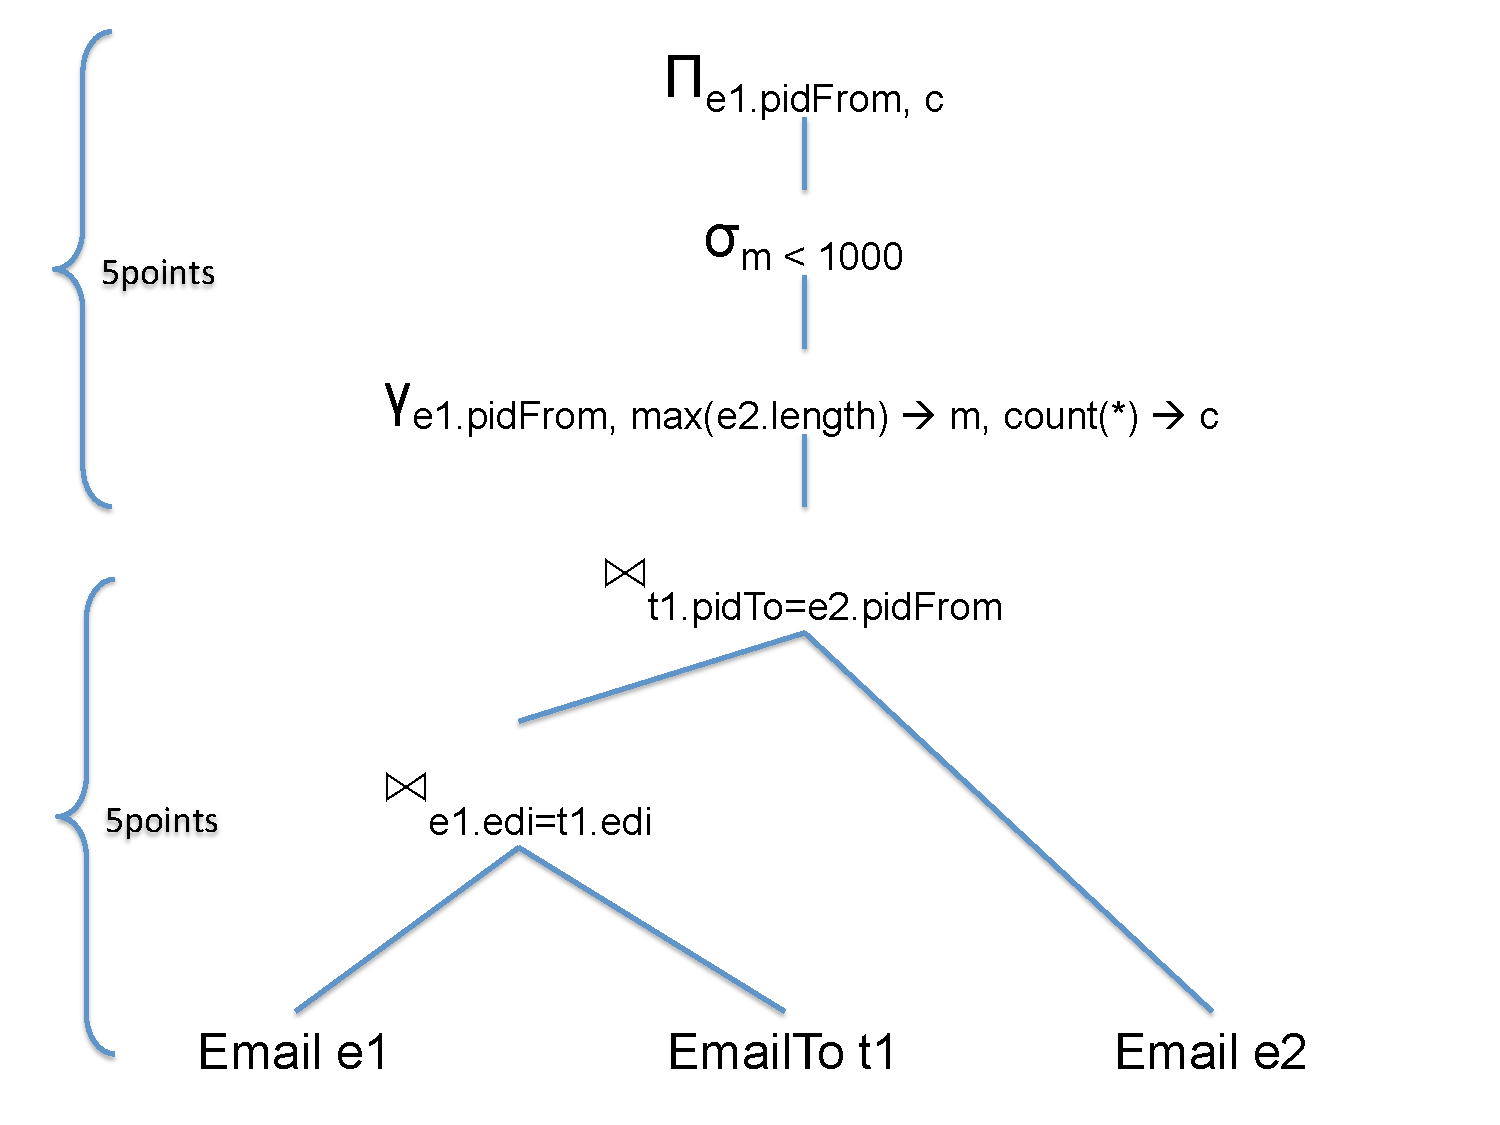
\includegraphics[width=.99\textwidth]{FIGS/problem1e-ra.pdf}}
\end{solution}


\newpage

{\scriptsize
\hfill
\begin{tabular}{l}
\texttt{Person(\underline{pid},name)} \\
\texttt{Email(\underline{eid}, pidFrom, tid, body, length)} \\
\texttt{EmailTo(eid,pidTo)}
\end{tabular}
}

\part[10] The query below retrieves all emails where every recipient
was named Alice.  Write a query plan in the relational algebra for
this query.

\begin{verbatim}
          select e1.eid
          from Email e1
          where not exists (select *
                            from EmailTo e2, Person p
                            where e1.eid = e2.eid
                              and e2.pidTo = p.pid
                              and p.name != 'Alice');
\end{verbatim}

\underline{\bf Answer} (write a  query plan; you may draw it as a tree):

\vfill

\begin{solution}

  \centerline{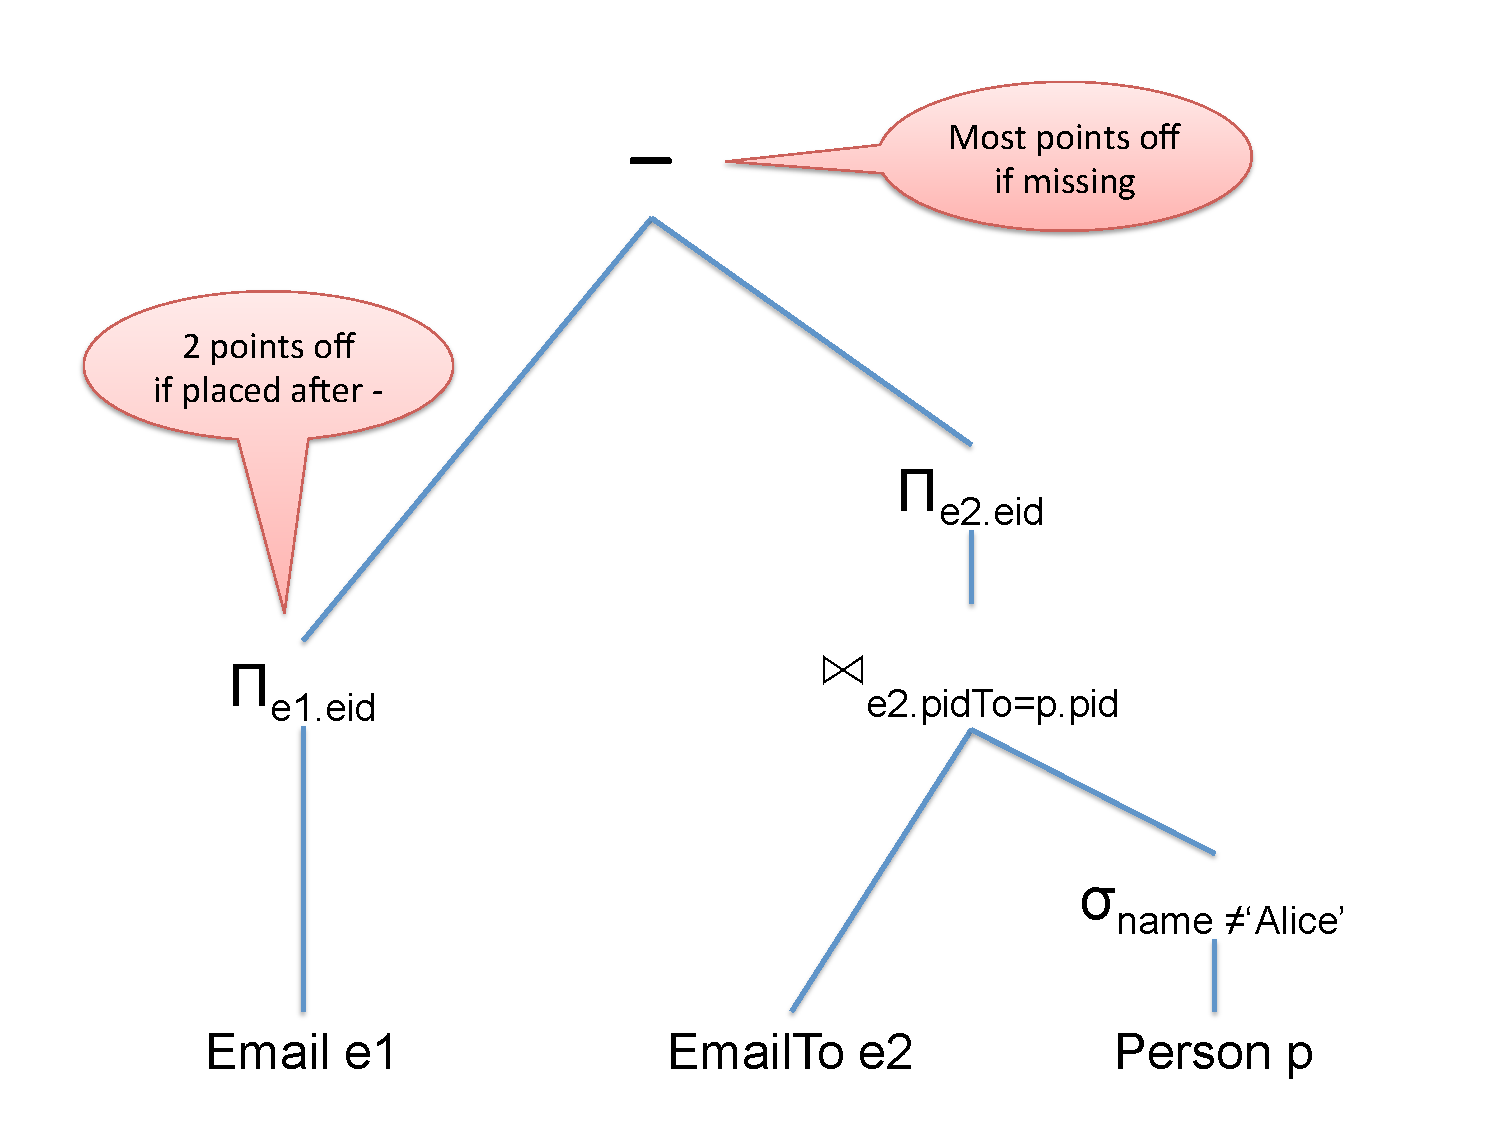
\includegraphics[width=.99\textwidth]{FIGS/problem1f-ra.pdf}}
\end{solution}


\end{parts}

\newpage




\section{XML/XPath/XQuery}

\question (\totalpoints\ points) 



The following DTD describes an XML document about students and the
courses they take:


\begin{verbatim}
<!DOCTYPE Enrollment [
	<!ELEMENT Enrollment  (student* )>
	<!ELEMENT student  (name,  address, course*)>
	<!ELEMENT course  (title, instructor, grade?)>
	<!ELEMENT name  (#PCDATA )>
	<!ELEMENT address (#PCDATA )>
	<!ELEMENT title  (#PCDATA )>
	<!ELEMENT instructor  (#PCDATA )>
	<!ELEMENT grade  (#PCDATA )>
]>
\end{verbatim}


\begin{parts}
  \part[10] Write an XPath expression that retrieves the names of all
  students whose address is 'Seattle' and who received a grade $<
  3.0$.  You should assume that the query processor performs the
  correct type conversions: that is, is suffices for you to write
  $\texttt{grade}<3.0$.

\underline{\bf Answer} (write a XPath expression):

\vfill

\begin{solution}
{\footnotesize
\begin{verbatim}
doc("problem2.xml")/Enrollment/student[address='Seattle'][course/grade<3.0]/name
\end{verbatim}
}
Notes:
\begin{itemize}
\item 1-2 points off for syntax errors.
\item 2 points off for XQuery instead of XPath.
\end{itemize}

\end{solution}

\newpage


  \part[10] The data is not normalized: the same course is listed
  multiple times, once for each student who took that course.  You
  normalize the data and represent it as follows:
%
\begin{verbatim}
<!DOCTYPE Normalized [
	<!ELEMENT Normalized  (students,courses,takes)>
	<!ELEMENT students  (student* )>
	<!ELEMENT courses   (course* )>
	<!ELEMENT takes   (take* )>
	<!ELEMENT student   (name, address)>
        <!ELEMENT course    (title, instructor)>
        <!ELEMENT take    (name, title, grade?)>
]>
\end{verbatim}
%
  Your Boss does not understand data anomalies and normalization
  theory, so he asks you to convert it back to the orignal format.
  Write an XQuery that transforms the \texttt{Normalized} data to the
  \texttt{Enrollment} data.

\underline{\bf Answer} (write a XPath expression):

\vfill

\begin{solution}

\begin{verbatim}
<Enrollment>
  { for $n in doc("problem2b.xml")/Normalized,
    $s in $n/students/student
    return <student>
             { $s/name,
               $s/address,
               for $e in $n/takes/take[name=$s/name],
                   $c in $n/courses/course[title=$e/title]
               return <course>
                        { $c/title,
                          $c/instructor,
                          $e/grade
                        }
                      </course>
              }
           </student>
   }
</Enrollment>
\end{verbatim}
Notes:
\begin{itemize}
\item 2-3 points were taken of for missing joins.
\end{itemize}
\end{solution}


\end{parts}

\newpage

\section{E/R Diagrams, Constraaints, Conceptual Design}

\question (\totalpoints\ points) 

\begin{parts}
  \part[10] The following E/R diagram describes a database about
  students and teachers:

\centerline{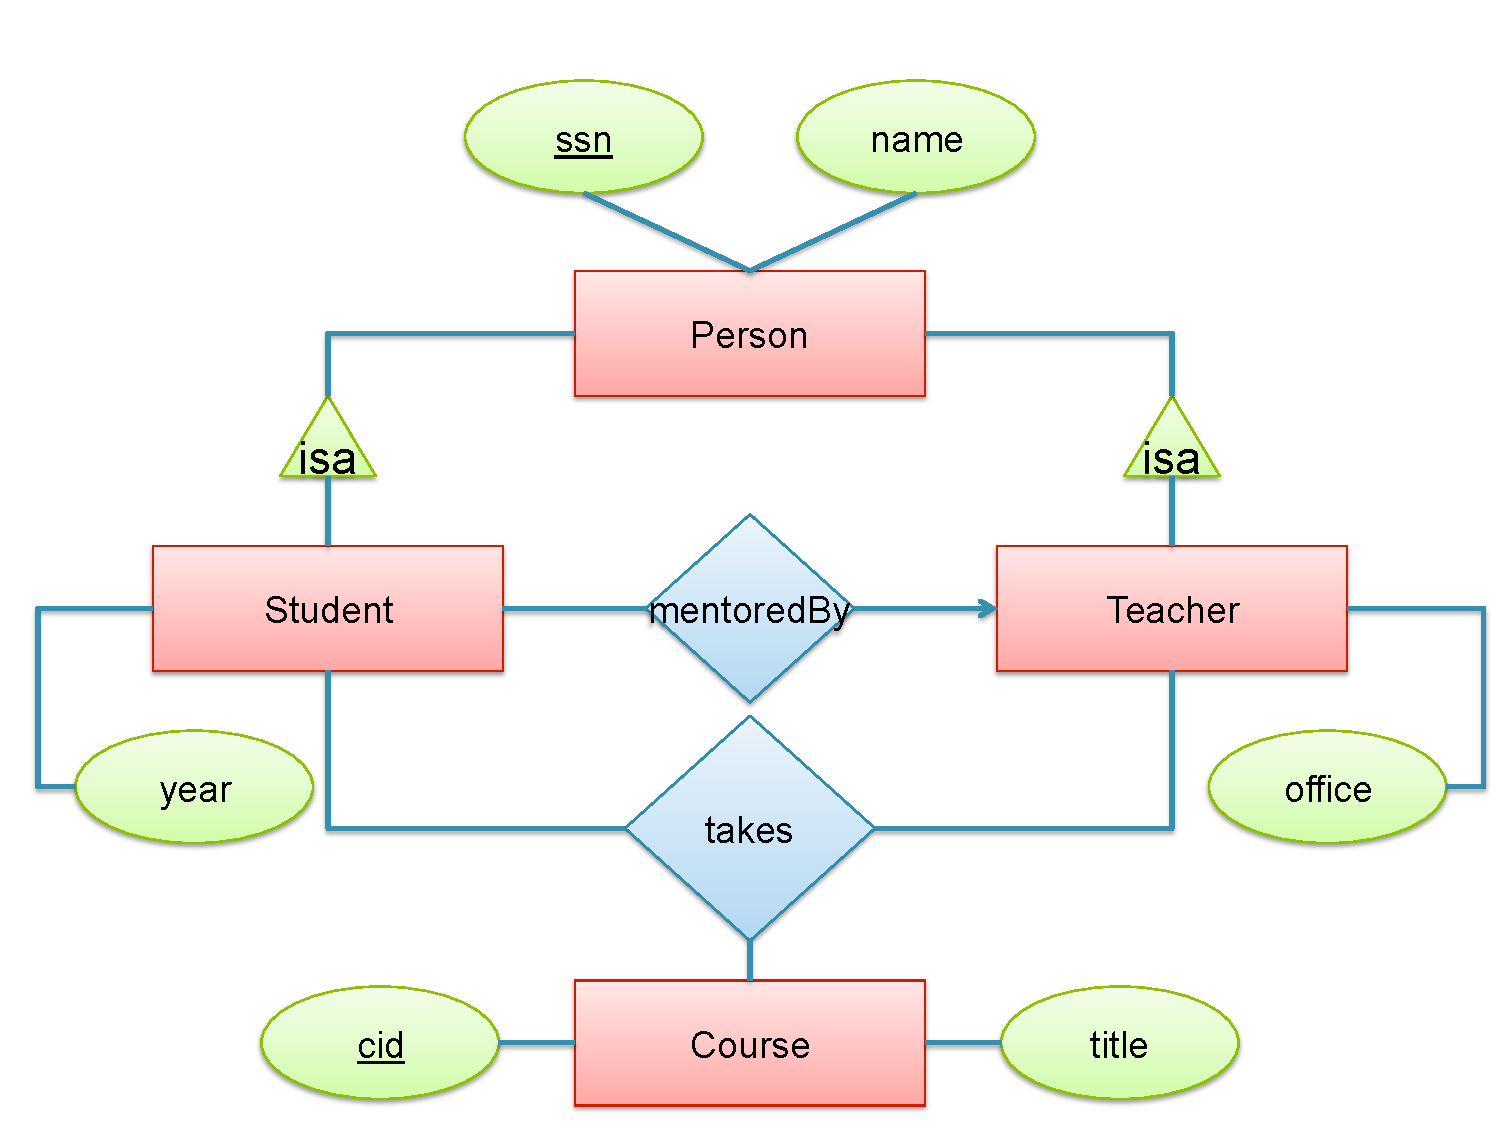
\includegraphics[width=.99\textwidth]{FIGS/er-figure}}

Every student and every teacher is a person.  Some students have a
teacher mentor.  Every student is in some year (1, 2, 3, \ldots) and
every teacher has an office.  Students take courses from teachers.
Convert the E/R diagram to SQL.  You should choose appropriate data
types for all attributes, and should write all key and foreign key
constraints.

\newpage
\hfill 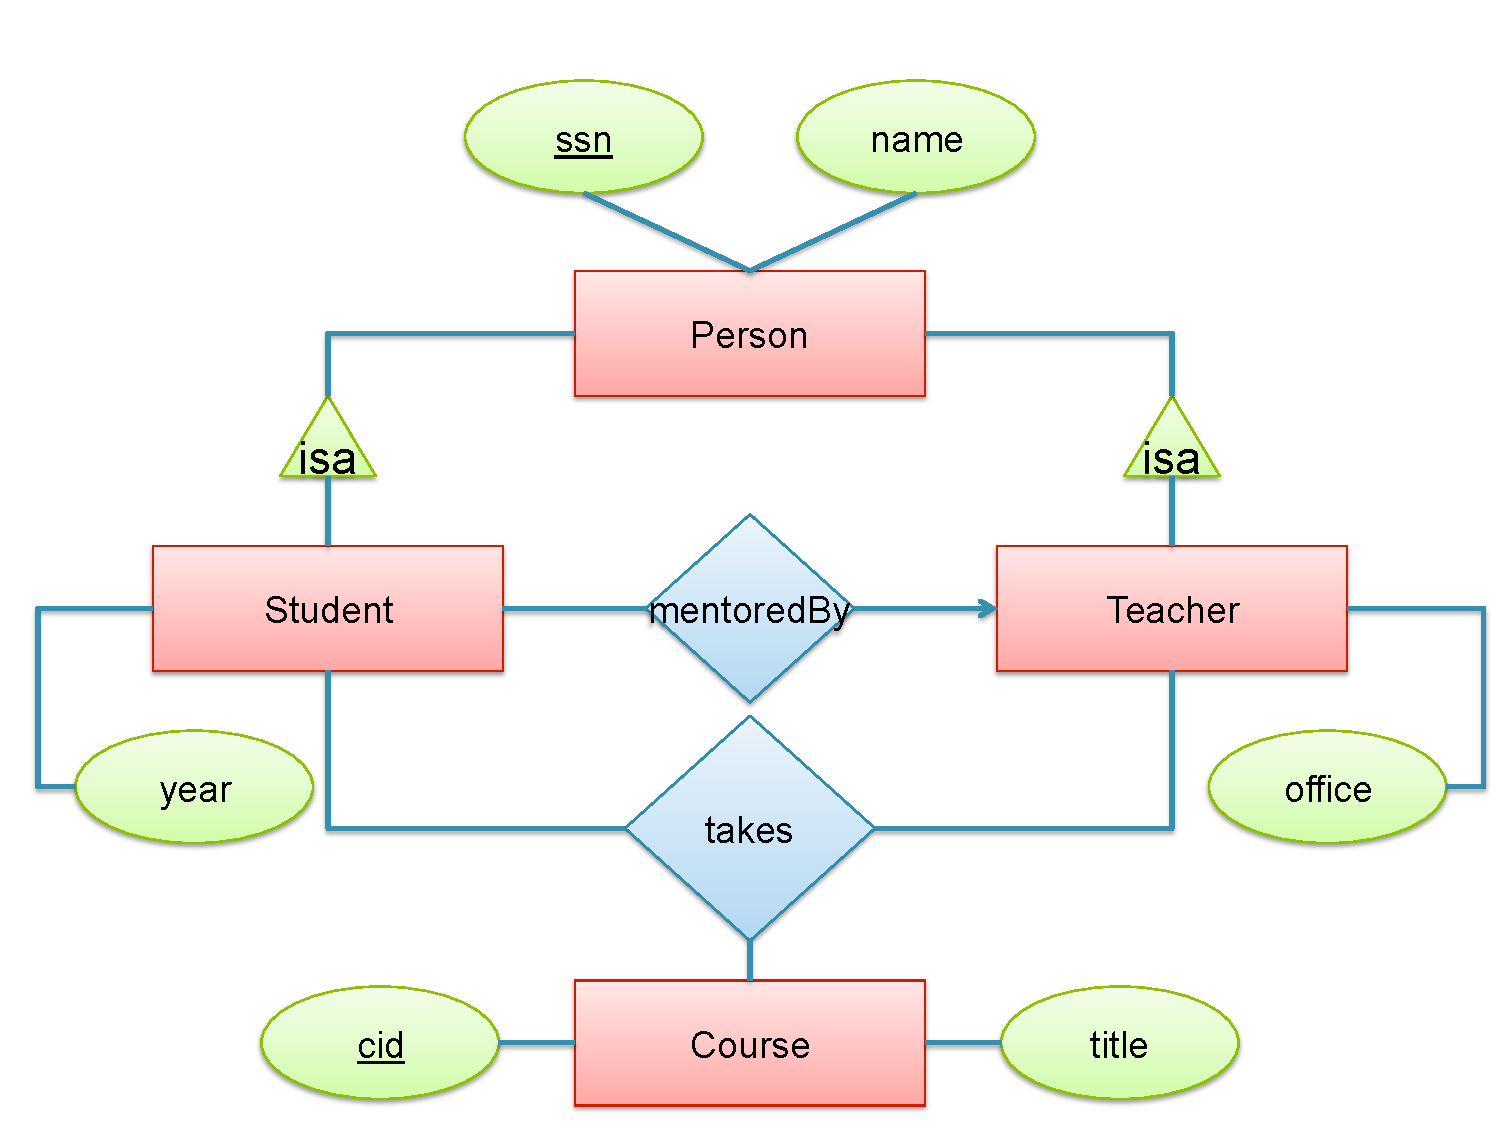
\includegraphics[width=.40\textwidth]{FIGS/er-figure}


\underline{\bf Answer} (Write CREATE TABLE statements):


\vfill

\begin{solution}
\begin{verbatim}
create table Person(ssn int primary key, name varchar(30));
create table Teacher(
        ssn int primary key references Person, 
        office varchar(20));
create table Student(
        ssn int primary key references Person, 
        mentoredby int references Teacher, 
        year int);
create table Course(cid int primary key, title varchar(30));
create table Takes(
        sid int references Student, 
        tid int references Teacher,
        cid int references Course);
\end{verbatim}
\end{solution}

\newpage

\part[10] Answer the following questions.

\begin{subparts}
  \subpart What is an update anomaly?  Choose one of the following:
  \begin{description}
  \item[(a)] One transaction reads an element that was updated by an
    earlier, uncommitted transaction.
  \item[(b)] The application wants to update a foreign key to a new
    value that does not exists in the referenced relation.
  \item[(c)] The same information is stored redundantly in the
    database, and only some, but not all copies are updated.
  \end{description}
  \answerline[(c)]{Answer (a), (b), or (c).}

\vspace{1cm}

  \subpart Every relational schema in SQL is in 1st normal form.
\answerline[true]{True or false?}

\vspace{1cm}

  \subpart Every XML data is in 1st normal form.
\answerline[false]{True or false?}

\vspace{1cm}

  \subpart Which of the following statements best describes the main
  reason for representing a relational database in 1st normal form?
  \begin{description}
  \item[(a)] To achieve physical data independence.
  \item[(b)] To remove data anomalies (insertion, update, deletion anomalies).
  \item[(c)] To save space on disk.
  \end{description}
\answerline[(a)]{Answer (a), (b), or (c).}

\vspace{1cm}

  \subpart Which of the following statements best describes the main
  reason for representing a relational database in BCNF?
  \begin{description}
  \item[(a)] To achieve physical data independence.
  \item[(b)] To remove data anomalies (insertion, update, deletion anomalies).
  \item[(c)] To save space on disk.
  \end{description}
\answerline[(b)]{Answer (a), (b), or (c).}

\end{subparts}

\newpage

\part[10] Consider the following instance of a relation $R(A,B,C,D)$:

\begin{tabular}{|c|c|c|c|}\hline\hline
$A$  & $B$  & $C$  & $D$ \\ \hline
$a$  & $b$  & $c$  & $d$ \\
$a'$ & $b$  & $c'$ & $d$ \\
$a'$ & $b'$ & $c$  & $d'$ \\ \hline
\end{tabular}

For each of the following statements indicate whether it is true or
false:

\begin{subparts}
  \subpart $A$ is a key.  \answerline[false]{True or false?}
  \subpart $B$ is a key.  \answerline[false]{True or false?}
  \subpart $AB$ is a key.  \answerline[true]{True or false?}
  \subpart $BD$ is a key.  \answerline[false]{True or false?}
  \subpart The functional dependency $A \rightarrow B$ holds.  \answerline[false]{True or false?}
  \subpart The functional dependency $B \rightarrow D$ holds.  \answerline[true]{True or false?}
  \subpart $D+ = BD$ holds.  \answerline[true]{True or false?}
\end{subparts}

\newpage

\part[10] Consider two relations $R(A,B,C,D)$ and $S(A,B,C,D)$, with
the following functional dependencies:

\begin{align*}
  & R: && A \rightarrow BCD \\
  &&& B \rightarrow ACD \\
\\
  & S: && BC \rightarrow AD \\
  &&& D \rightarrow B
\end{align*}

\begin{subparts}
  \vfill

  \subpart Find all keys in $R$.  \answerline[$A$ and $B$]{The keys are:} 

  \vfill

  \subpart Find all keys in $S$. \answerline[$BC$ and $CD$]{The keys
    are:}

  \vfill

  \subpart Find all keys in $R \cap S$. \answerline[$A$, $B$, and $CD$]{The keys are:}

   \begin{solution}
     A set of attribute is a superkey in $R \cap S$ iff it is a
     superkey in $R$ or in $S$.  The superkeys in $R$ are:
     $A,AC,AD,ACD, B,BC,BD,BCD, ABC,ABD, ABCD$.  The superkeys in $S$
     are: $BC, ABC, CD, ACD, BCD, ABCD$.  The superkeys in $R \cap S$
     are all them, and therefore the keys are $A$, $B$, and $CD$.
   \end{solution}

  \vfill

  \subpart Assume that the relations $R(A,B,C,D)$ and $S(A,B,C,D)$ do
  not have any common values.  That is, the values of the attribute
  $R.A$ are distinct from those of the attribute $S.A$, and the same
  for the attributes $B, C, D$.  Find all keys in $R \cup S$
  \answerline[$BC$ and $ACD$]{The keys are:}
  \begin{solution}
    A set of attributes is a superkey in $R \cup S$ iff it is a
    superkey in both $R$ and $S$. Thus, the superkeys in $R \cup S$
    are $BC, ABC, ACD, BCD, ABCD$.  The keys are: $BC$ and $ACD$.
  \end{solution}

  \vfill


\end{subparts}


\end{parts}

\newpage

\section{Transactions}

\question (\totalpoints\ points) 


\begin{parts}
  \part[30] Consider a database consisting of a single relation R:


\begin{tabular}{l|l|l|} \cline{2-3}
  R: & A & B \\  \cline{2-3}
     & 1 & 10 \\
     & 2 & 20 \\ \cline{2-3}
\end{tabular}

Three transactions run concurrently on this database, issuing commands
at the following time stamps:

\begin{tabular}{|c|l|l|l|} \hline
  Time & T1 & T2 & T3 \\ \hline
1 & begin transaction;              &                    & \\ \hline
2 & select * from R;                &                    & \\ \hline             
3 &                                 & begin transaction; & \\ \hline
4 &                                 & select * from R    & \\
  &                                 & where $A=2$;       & \\ \hline
% returns value 20
5 & update R set $B=30$             &                    & \\
  & where $A=2$;                    &                    & \\ \hline
6 &                                 &  select * from R   & \\
  &                                 &  where $A=2$;      & \\ \hline
% -- on sqlite: returns old value 20
% -- on sqlserver: waits until after time stamp 7
7 & commit;                         &                    & \\ \hline
% -- on sqlite: database is locked!  Need to retry on Step 11
% -- on sqlsever: success; T2 returns new value 30
8 &                                 &                    & begin transaction; \\ \hline
9 &                                 &                    & select * from R  \\
  &                                 &                    & where $A=2$; \\ \hline
% -- on sqlite: database is locked!  Need to retry on Step 12
% -- on sqlsever: success, returns new value 30
10 &                                & commit;            & \\ \hline
% -- success
11 & 
      % -- on sqlite only:
      % commit;
                                    &                     & \\ \hline
12 &                                &
                                       % -- on sqlite only
                                       % select * from R where A=2;
                                                          & \\ \hline
13 &                                &                     & commit; \\ \hline
% -- on sqlite: returns new value 30
\end{tabular}

Transaction T1 first reads the data, then updates the second record
($A=2$).  It attempts to commit at time stamp 7.

Transaction T2 attempts to read the second record ($A=2$) at time
stamp 4.

Transaction T3 attempts to read the second record ($A=2$) at time
stamp 9.

\newpage

\begin{subparts}
  \subpart Find out what happened.  You will consider two scenarios:
  when the database is managed with SQL Lite, and when the database is
  managed with SQL Server; in both cases the isolation level is set to
  SERIALIZABLE.  For each command issued by a transaction, indicate
  one of the following outcome:


\begin{description}
\item[SUCCESS] The request returns immediately, with success.  In this
  case you should write SUCCESS, and also write the value that the
  transaction has read, if applicable.
\item[ERROR] The request returns immediately, with error.  In this
  case you should write ERROR and indicate at which later time stamp
  the transaction needs to retry that command; if the command was a
  read, write down the value read by the transaction, when the command
  is reissued successfully.
\item[WAIT] The request causes the transaction to be placed on wait.
  In that case you should write WAIT, and also write at which later
  time stamp the transaction will be allowed to resume; if the command
  was a read, write down the value read by the transaction, when the
  command is resumed.
\end{description}

For example, you may answer as follows (not a real answer):

\vspace{2cm}

\begin{center} 
{\footnotesize
\begin{tabular}{|c|l|l|l|} \hline
  Time & T1 & T2 & T3 \\ \hline
1 & begin transaction;              &                    & \\ \hline
2 & select * from R;                &                    & \\
  & -- WAIT UNTIL $T=4$             &                    & \\ \hline
3 &                                 & begin transaction; & \\
  &                                 & -- SUCCESS         & \\ \hline
4 &                                 & select * from R    & \\
  &                                 & where $A=2$;       & \\ 
  &                                 & -- SUCCES: value$=30$   & \\
  & -- RESUMED: values$10,30$       &                    & \\ \hline
  &                                 &                    & \\
  &                                 &                    & \\
  & \ldots                          & \ldots             & \ldots \\
  &                                 &                    & \\
  &                                 &                    & \\  \hline
% -- on sqlite: returns new value 30
\end{tabular}
}
\end{center}


\newpage

\hspace{-3cm}
\begin{tabular}{|c|l|l|l|} \hline
 \multicolumn{4}{|c|}{This schedule is excecuted on {\bf SQL Lite}} \\ \hline
   & \parbox{0.32\textwidth}{T1} & \parbox{0.32\textwidth}{T2} & \parbox{0.32\textwidth}{T3} \\ \hline
% ------------------------------------------------------------------
  &                                 &                    & \\
1 & begin transaction;              &                    & \\
  &                                 &                    & \\ \hline
% ------------------------------------------------------------------
  &                                 &                    & \\
2 & select * from R;                &                    & \\
  &                                 &                    & \\ \hline
% ------------------------------------------------------------------
  &                                 &                    & \\
3 &                                 & begin transaction; & \\
  &                                 &                    & \\ \hline
% ------------------------------------------------------------------
  &                                 &                    & \\
4 &                                 & select * from R    & \\
  &                                 & where $A=2$;       & \\
% returns value 20
  &                                 &                    & \\ \hline
% ------------------------------------------------------------------
  &                                 &                    & \\
5 & update R set $B=30$             &                    & \\
  & where $A=2$;                    &                    & \\
  &                                 &                    & \\ \hline
% ------------------------------------------------------------------
  &                                 &                    & \\
6 &                                 &  select * from R   & \\
  &                                 &  where $A=2$;      & \\
  &                                 &                    & \\ \hline
% -- on sqlite: returns old value 20
% -- on sqlserver: waits until after time stamp 7
% ------------------------------------------------------------------
  &                                 &                    & \\
7 & commit;                         &                    & \\
  &                                 &                    & \\ \hline
% -- on sqlite: database is locked!  Need to retry on Step 11
% -- on sqlsever: success; T2 returns new value 30
% ------------------------------------------------------------------
  &                                 &                    & \\
8 &                                 &                    & begin transaction; \\
  &                                 &                    & \\ \hline
  &                                 &                    & \\
% ------------------------------------------------------------------
9 &                                 &                    & select * from R  \\
  &                                 &                    & where $A=2$; \\
  &                                 &                    & \\ \hline
% -- on sqlite: database is locked!  Need to retry on Step 12
% -- on sqlsever: success, returns new value 30
  &                                 &                    & \\
% ------------------------------------------------------------------
10 &                                & commit;            & \\
  &                                 &                    & \\ \hline
% -- success
  &                                 &                    & \\
% ------------------------------------------------------------------
11 & 
      % -- on sqlite only:
      % commit;
                                    &                     & \\
  &                                 &                    & \\ \hline
  &                                 &                    & \\
                                       % -- on sqlite only
                                       % select * from R where A=2;
% ------------------------------------------------------------------
12 &                                &
                                                          & \\ \hline
% ------------------------------------------------------------------
13 &                                &                     & commit; \\
  &                                 &                    & \\ \hline
% -- on sqlite: returns new value 30
% ------------------------------------------------------------------
\end{tabular}

  \begin{solution}

{\scriptsize
\begin{tabular}{|c|l|l|l|} \hline
  Time & T1 & T2 & T3 \\ \hline
1 & begin transaction;              &                    & \\ \hline
2 & select * from R;                &                    & \\
  & -- SUCCESS: values 10,20           &                    & \\ \hline
3 &                                 & begin transaction; & \\ \hline
4 &                                 & select * from R    & \\
  &                                 & where $A=2$;       & \\ 
  &                                 & -- SUCCES: value 20   & \\ \hline
5 & update R set $B=30$             &                    & \\
  & where $A=2$;                    &                    & \\
  & -- SUCCESS                         &                    & \\ \hline
6 &                                 &  select * from R   & \\
  &                                 &  where $A=2$;      & \\
  &                                 & -- SUCCES: value 20   & \\ \hline
% -- on sqlite: returns old value 20
% -- on sqlserver: waits until after time stamp 7
7 & commit;                         &                    & \\
  & ERROR: retry on 11              &                    & \\ \hline
% -- on sqlite: database is locked!  Need to retry on Step 11
% -- on sqlsever: success; T2 returns new value 30
8 &                                 &                    & begin transaction; \\
  &                                 &                    & SUCCESS  \\ \hline
9 &                                 &                    & select * from R  \\
  &                                 &                    & where $A=2$; \\
  &                                 &                    & ERROR: retry on 12 \\ \hline
% -- on sqlite: database is locked!  Need to retry on Step 12
% -- on sqlsever: success, returns new value 30
10 &                                & commit;            & \\
  &                                 & -- SUCCES:            & \\ \hline
% -- success
11 & -- REISSUE:                    &                     & \\
   & commit;                        &                     & \\
   & -- SUCCESS;                    &                    & \\ \hline
12 &                                &                    & -- REISSUE: \\
   &                                &                    & select * from R where $A=2$; \\
   &                                &                    & -- SUCCESS: value 30 \\ \hline
13 &                                &                     & commit; \\
   &                                &                     & -- SUCCESS \\ \hline
% -- on sqlite: returns new value 30
\end{tabular}
}

  \end{solution}

\newpage

\hspace{-3cm}
\begin{tabular}{|c|l|l|l|} \hline
 \multicolumn{4}{c|}{This schedule is excecuted on {\bf SQL Server}} \\ \hline
   & \parbox{0.32\textwidth}{T1} & \parbox{0.32\textwidth}{T2} & \parbox{0.32\textwidth}{T3} \\ \hline
% ------------------------------------------------------------------
  &                                 &                    & \\
1 & begin transaction;              &                    & \\
  &                                 &                    & \\ \hline
% ------------------------------------------------------------------
  &                                 &                    & \\
2 & select * from R;                &                    & \\
  &                                 &                    & \\ \hline
% ------------------------------------------------------------------
  &                                 &                    & \\
3 &                                 & begin transaction; & \\
  &                                 &                    & \\ \hline
% ------------------------------------------------------------------
  &                                 &                    & \\
4 &                                 & select * from R    & \\
  &                                 & where $A=2$;       & \\
% returns value 20
  &                                 &                    & \\ \hline
% ------------------------------------------------------------------
  &                                 &                    & \\
5 & update R set $B=30$             &                    & \\
  & where $A=2$;                    &                    & \\
  &                                 &                    & \\ \hline
% ------------------------------------------------------------------
  &                                 &                    & \\
6 &                                 &  select * from R   & \\
  &                                 &  where $A=2$;      & \\
  &                                 &                    & \\ \hline
% -- on sqlite: returns old value 20
% -- on sqlserver: waits until after time stamp 7
% ------------------------------------------------------------------
  &                                 &                    & \\
7 & commit;                         &                    & \\
  &                                 &                    & \\ \hline
% -- on sqlite: database is locked!  Need to retry on Step 11
% -- on sqlsever: success; T2 returns new value 30
% ------------------------------------------------------------------
  &                                 &                    & \\
8 &                                 &                    & begin transaction; \\
  &                                 &                    & \\ \hline
  &                                 &                    & \\
% ------------------------------------------------------------------
9 &                                 &                    & select * from R  \\
  &                                 &                    & where $A=2$; \\
  &                                 &                    & \\ \hline
% -- on sqlite: database is locked!  Need to retry on Step 12
% -- on sqlsever: success, returns new value 30
  &                                 &                    & \\
% ------------------------------------------------------------------
10 &                                & commit;            & \\
  &                                 &                    & \\ \hline
% -- success
  &                                 &                    & \\
% ------------------------------------------------------------------
11 & 
      % -- on sqlite only:
      % commit;
                                    &                     & \\
  &                                 &                    & \\ \hline
  &                                 &                    & \\
                                       % -- on sqlite only
                                       % select * from R where A=2;
% ------------------------------------------------------------------
12 &                                &
                                                          & \\ \hline
% ------------------------------------------------------------------
13 &                                &                     & commit; \\
  &                                 &                    & \\ \hline
% -- on sqlite: returns new value 30
% ------------------------------------------------------------------
\end{tabular}

  \begin{solution}

{\scriptsize
\begin{tabular}{|c|l|l|l|} \hline
  Time & T1 & T2 & T3 \\ \hline
1 & begin transaction;              &                    & \\ \hline
2 & select * from R;                &                    & \\
  & -- SUCCESS: values 10,20           &                    & \\ \hline
3 &                                 & begin transaction; & \\ \hline
4 &                                 & select * from R    & \\
  &                                 & where $A=2$;       & \\ 
  &                                 & -- SUCCES: value 20   & \\ \hline
5 & update R set $B=30$             &                    & \\
  & where $A=2$;                    &                    & \\
  & -- SUCCESS                         &                    & \\ \hline
6 &                                 &  select * from R   & \\
  &                                 &  where $A=2$;      & \\
  &                                 & -- WAIT: until 7   & \\ \hline
% -- on sqlite: returns old value 20
% -- on sqlserver: waits until after time stamp 7
7 & commit;                         &                    & \\
  & -- SUCCESS                      &                    & \\
  &                                 & -- SUCCCESS: value 30 & \\ \hline
% -- on sqlite: database is locked!  Need to retry on Step 11
% -- on sqlsever: success; T2 returns new value 30
8 &                                 &                    & begin transaction; \\
  &                                 &                    & -- SUCCESS  \\ \hline
9 &                                 &                    & select * from R  \\
  &                                 &                    & where $A=2$; \\
  &                                 &                    & -- SUCCESS: value 30 \\ \hline
% -- on sqlite: database is locked!  Need to retry on Step 12
% -- on sqlsever: success, returns new value 30
10 &                                & commit;            & \\
  &                                 & -- SUCCES:            & \\ \hline
% -- success
11 &                                &                    & \\ \hline
12 &                                &                    & \\ \hline
13 &                                &                     & commit; \\
   &                                &                     & -- SUCCESS \\ \hline
% -- on sqlite: returns new value 30
\end{tabular}
}
\end{solution}

\subpart What is the serialization order of the three transactions on
SQL Lite? \answerline[T2, T1, T3]{Give an order or the transactions
  T1, T2, T3:}

\vfill

\subpart What is the serialization order of the three transactions on
SQL Server? \answerline[T1, T2, T3]{Give an order or the transactions
  T1, T2, T3:}

\vfill

\end{subparts}

\newpage

\part[10] Recall that a {\em shared lock} (or {\em read lock}) may be
held by several transactions, while an {\em exclusive lock} (or {\em
  write lock}) can be held by only one transaction. 
%
\begin{itemize}
\item System A uses shared and exclusive locks.
\item System B uses only exclusive locks.
\end{itemize}
%
Indicate which statements below are true.

\begin{subparts}
  \vfill

  \subpart System A may be able to execute more transactions per
  second than system B. \answerline[true]{True or false?}

  \vfill

  \subpart If all transactions are read-only, then on system A no
  transaction ever waits. \answerline[true]{True or false?}

  \vfill

  \subpart If all transactions are write-only, then on system B no
  transaction ever waits. \answerline[false]{True or false?}

  \vfill

  \subpart There exists schedules that result in a deadlock on system
  A but not in a deadlock on system B. \answerline[true]{True or
    false?}
  \begin{solution}
    True.  For example the following schedule: Start1, Start2,
    Read1(X), Read2(X), Write1(X), Write2(X), Commit1, Commit2.  On
    system A, both transactions start with a read lock on X, then
    attempt to escalate it to a write lock, and result in deadlock.
    On system B, the second transaction is placed on wait during the
    operation Read2(X).
  \end{solution}

  \vfill
\end{subparts}



\newpage

\part[10] A {\em static database} is a database where no insertions or
deletions are performed.  A {\em dynamic database} is a database that
allows insertions and deletions.  We consider a scheduler that has one
lock for each record in the database (like SQL Server).  Answer the
questions below:

\begin{subparts}

  \subpart In a static database, strict two phase locking guarantees
  that the schedule is serializable while two phase locking does not.
  \answerline[false]{True or false}

  \vfill

  \subpart Strict two phase locking guarantees that the schedule is
  recoverable, while two phase locking does
  not. \answerline[true]{True or false}

  \vfill

  \subpart In a dynamic database, strict two phase locking can prevent
  phantoms, while two phase locking cannot. \answerline[false: needs
  table lock]{True or false}

  \vfill

  \subpart Strict two phase locking is more difficult to implement and
  most database system do not support it. \answerline[false]{True or
    false}

  \vfill

  \subpart Strict two phase locking holds all the locks until the end
  of a transaction, while two phase locking may release the locks
  earlier. \answerline[true]{True or false}

  \vfill

%   \subpart Two phase locking is called this way because it uses two
%   locks for each record: a shared lock and an exclusive
%   lock. \answerline[false]{True or false}
% 
%   \vfill

\newpage

  \subpart In both two phase locking and strict two phase locking all
  locks must precede all unlocks. \answerline[true]{True or false}

  \vfill

  \subpart In strict two phase locking deadlocks are not possible,
  while in two phase locking deadlocks are
  possible. \answerline[false]{True or false}

  \vfill

  \subpart If the database uses shared locks for read operations, then
  if all transactions are read-only then no deadlocks are possible.
  \answerline[true]{True or false}

  \vfill

  \subpart SQL Server checks for deadlocks at regular intervals, and
  if it detects a deadlock then aborts a transaction
  \answerline[true]{True or false}

  \vfill

  \subpart Suppose that the table $R$ has 1000 records.  Then the
  transaction below needs to acquire 1000 locks:

\begin{verbatim}
       begin transaction;
       select * from R;
       commit;
\end{verbatim}
  \answerline[true]{True or false}



\end{subparts}


\end{parts}

\newpage

\section{Parallel Data Processing}

\question (\totalpoints\ points) 


\begin{parts}
  \part[10] We have a large database, on which we need to run
  repeatedly SQL queries.  Each SQL query has up to 5 joins, a
  group-by, and some selections.  We use a parallel database system,
  and we consider the following alternative evaluation strategies: (a)
  inter-query parallelism, (b) inter-operator parallelism, (c)
  intra-operator parallelism.  In each case we deploy only one
  strategy, i.e. we do not combine them.  Consider a job $J$
  consisting of several SQL queries, and assume it has the following
  running time:

  \begin{itemize}
  \item Job $J$ runs in $T=100$ minutes on 10 nodes.
  \end{itemize}

  Estimate the running time of that job if we increase the number of
  nodes from 10 to 100, in each of the six cases below.  In each case,
  assume that the database is capable of delivering linear speedup,
  when the execution strategy is parallelizable.

\vfill

\begin{center}
  \begin{tabular}{|l||l|l|l|} \hline
    \multicolumn{4}{|c|}{} \\
    \multicolumn{4}{|c|}{\bf Write the running time $T$ on 100 nodes} \\
    \multicolumn{4}{|c|}{} \\ \hline Job $J$ &
    \multicolumn{3}{c|}{Type of Parallelism} \\ \cline{2-4} consists
    of: & Inter-query & Inter-operator & Intra-operator \\ \hline
    &      &      &    \\
    1 SQL query &      &      &    \\
    & & & \\ \hline
    &      &      &    \\
    1000 SQL queries & &      &    \\
    & & & \\ \hline
  \end{tabular}
\end{center}

\vfill

\begin{solution}
  \begin{tabular}{|l||l|l|l|} \hline Job $J$ &
    \multicolumn{3}{c|}{Type of Parallelism} \\ \cline{2-4} consists
    of: & Inter-query & Inter-operator & Intra-operator \\ \hline 1
    SQL query & 100 & 100 & 10 \\ \hline 1000 SQL queries & 10 & 100 &
    10 \\ \hline
  \end{tabular}
\end{solution}

\vfill

\newpage

\part[10] The query below computes the total number of customers with
any given date of birth:

\begin{verbatim}
           select birthdate, count(*)
           from Customer x
           group by x.birthdate
\end{verbatim}

The attributes \texttt{birthdate} represents the date of birth of the
customer: it contains the day and month only (not the year!).  We
evaluate the query using Map-Reduce. Assume:

\begin{itemize}
\item The relation \texttt{Customer} has 16MB
\end{itemize}

We consider choosing the block size to be one of the following three
values: 128KB, 64KB, 32KB.  (Recall that $1MB = 1024KB$; thus, if the
block size is 128KB, then the \texttt{Customer} file has $16\cdot
1024/128 = 128$ blocks.)  Indicate the maximum number of instances
that you can use and still achieve linear speedup, if the data is
uniformly distributed.  Assume that the number of map tasks is equal
to the number of blocks, and that the number of reduce tasks is set to
the number of instances.

\begin{subparts}
  \vfill

  \subpart The block size is 128KB.  \answerline[$16MB/128KB =
  128$]{Maximum number of instances:}

  \vfill

  \subpart The block size is 64KB.  \answerline[$16MB/64KB =
  256$]{Maximum number of instances:}

  \vfill

  \subpart The block size is 32KB.  \answerline[365: \#
  days/year]{Maximum number of instances:}

  \vfill

\end{subparts}

\newpage

\part[10] A Map/Reduce Job runs on 10 instances, and uses 100 Map
Tasks and 50 Reduce Tasks.  The input file has 5GB, and the block size
is 50K.  We assume that the map function produces an output whose size
is approximatively equal to that of the input: in other words, the
size of the intermediate result is also 5GB.

\begin{subparts}

  \vfill

  \subpart What is the total number of intermediate files to which the
  mappers write their outputs?  \answerline[$50\cdot 100 =
  5000$]{Write the number of files:}

  \vfill

  \subpart After a reducer copies, it needs to sort.  How large is the
  file that needs to be sorted?  Answer with the expected value.
  \answerline[$5GB/50 = 100MB$]{Write the size of the file:}

  \vfill

  \subpart At any time, one instance runs only one map task, or only
  one reduce task.  Suppose that a map task takes 1 minute to finish,
  and a reduce task also takes 1 minute to finish.  What is the total
  running time for the Map/Reduce job?  \answerline[$100\frac{1}{10} +
  50\frac{1}{10} = 15$minutes]{Write the time in minutes:}

  \vfill

  \subpart Continue to assume that each map task and each reduce task
  takes 1 minute.  However, one single map task exhibits a skew, and
  take 10 minutes to complete instead of 1 minute; all other 99 map
  tasks still take 1 minute.  What is the total running time for the
  Map/Reduce job?  \answerline[$15+9=24$ minutes]{Write the time in
    minutes:}

  \vfill

    \end{subparts}


\end{parts}

% \newpage
% 
% \section{Database as a Service}
% 
% \question (\totalpoints\ points) 
% 
% OLD STUFF
% 
% \begin{parts}
%   \part[5] Consider the following two words:
% \end{parts}

\end{questions}


\end{document}
